\section{Methods} \label{sec:methods}

\begin{figure*}
  \centering
  \begin{subfigure}[t]{0.43\linewidth}
    \centering
  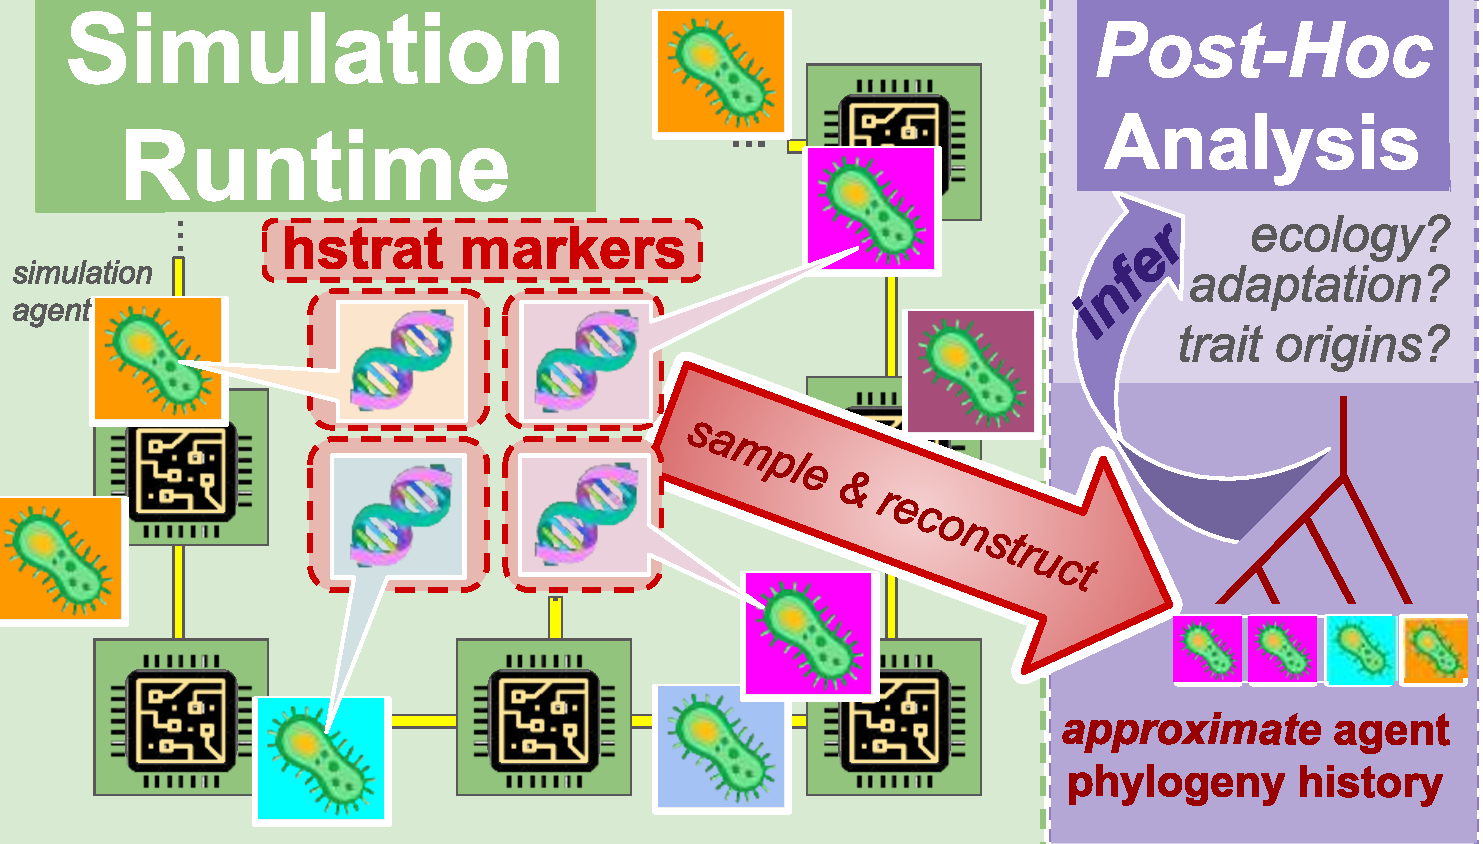
\includegraphics[width=\linewidth]{binder-wse-sketches/tex-access-proposal/img/runtime-posthoc-schematic}
    \caption{\footnotesize %
    hstrat markers help reconstruct phylogenies, which can tell evolutionary dynamics.
    }
    \label{fig:runtime-posthoc-schematic}
  \end{subfigure}
  \hspace{0.07\linewidth}
  \begin{subfigure}[t]{0.43\linewidth}
    \centering
  \includegraphics[width=\linewidth]{binder-wse-sketches/tex-access-proposal/img/async-ga-schematic}
    \caption{\footnotesize WSE island model evolutionary algorithm implementation.}
    \label{fig:async-ga-schematic}
  \end{subfigure}

\caption{%
\textbf{Methods for trackable distributed evolution simulation.}
\footnotesize
Subfigure \ref{fig:runtime-posthoc-schematic} shows use of hstrat markers to for reconstruct-based phylogenetic tracking of highly-distributed evolution simulations.
Subfigure \ref{fig:async-ga-schematic} summarizes asynchronous, callback-based approach to population exchange (``migration''') used to instantiate evolving populations across WSE PEs.
}
\label{fig:schematic}

\end{figure*}


\begin{figure}[b!]
  \centering
  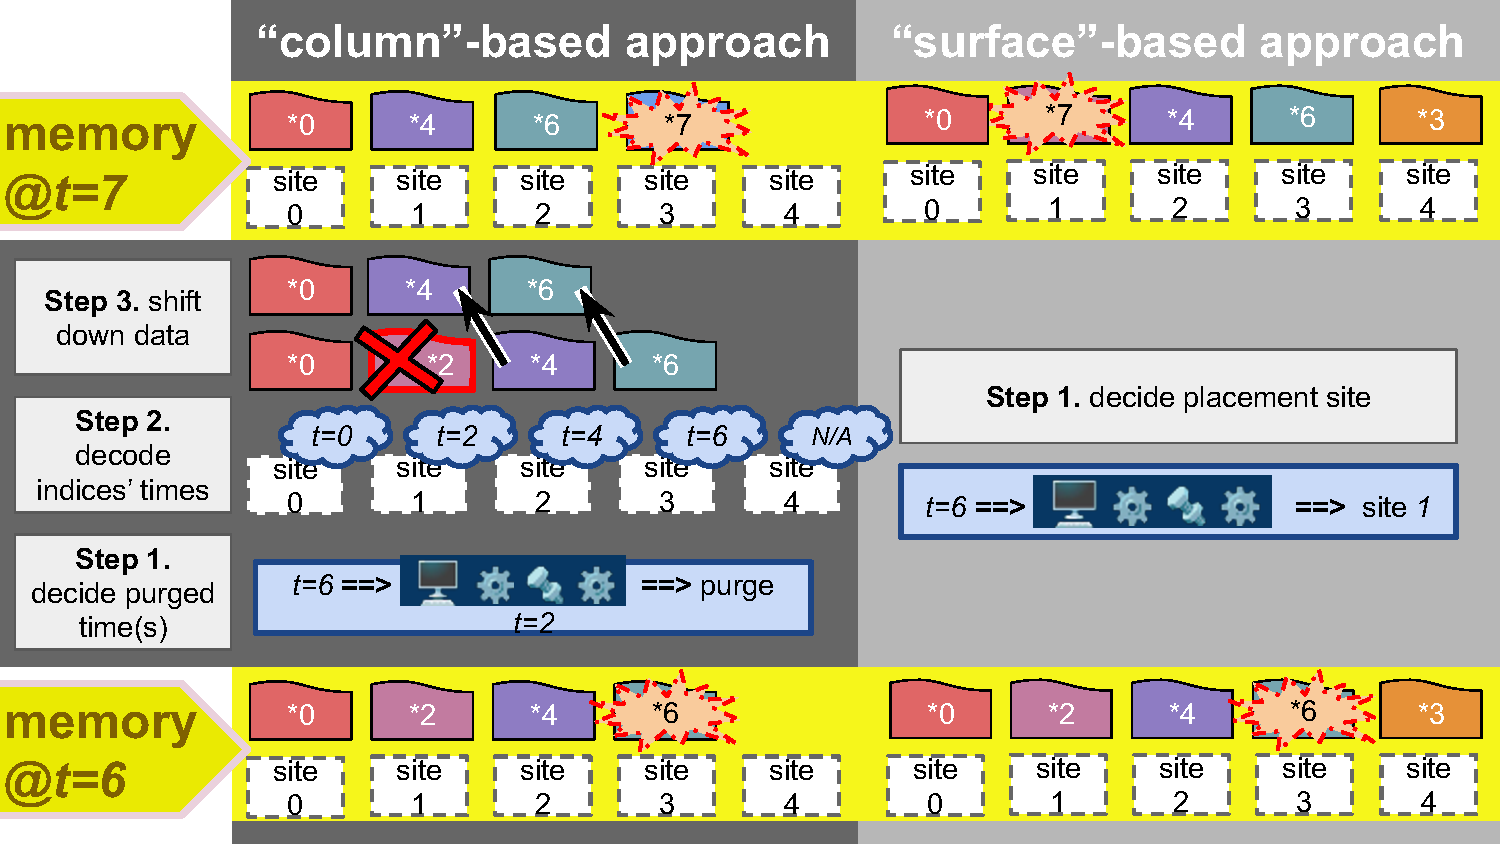
\includegraphics[width=0.95\linewidth]{img/surf-vs-column-schematic}

  \vspace{-1.5ex}

  \caption{
  \textbf{Column vs. surface-based hereditary stratigraphy.}
  \footnotesize
  Contrast of existing sorted-order ``column''-based stratum retention framework with proposed explicitly addressed ``surface''-based approach.}
  \label{fig:surf-vs-column-schematic}
  \vspace{-0.2in}
\end{figure}


\begin{figure*}
  \centering
\begin{subfigure}[b]{0.43\linewidth}
\centering
\textbf{steady retention policy}
\end{subfigure}
\begin{subfigure}[b]{0.43\linewidth}
\centering
\textbf{tilted retention policy}
\end{subfigure}

  \begin{subfigure}[b]{0.43\linewidth}
    \centering
  \includegraphics[height=\linewidth,angle=90,trim={0 2.4cm 0 0},clip]{binder-surface-concept/teeplots/10/cnorm=log+num-generations=4096+surface-size=256+viz=site-deposition-depth-by-rank-heatmap+ynorm=linear+ext=}
    \caption{256 bit steady surface site age plot}
    % \label{fig:runtime-posthoc-schematic}
  \end{subfigure}
  \begin{subfigure}[b]{0.43\linewidth}
    \centering
  \includegraphics[height=\linewidth,angle=90, trim={0 0 0 2.4cm},clip]{binder-surface-concept/teeplots/21/cnorm=log+num-generations=4096+surface-size=256+viz=site-deposition-depth-by-rank-heatmap+ynorm=linear+ext=}
    \caption{256 bit tilted surface site age plot}
    % \label{fig:async-ga-schematic}
  \end{subfigure}


\begin{subfigure}[b]{0.43\linewidth}
  \centering
\includegraphics[width=\linewidth,trim={0 0 0 0},clip]{binder-surface-concept/teeplots/10/num-generations=262144+surface-size=64+viz=stratum-persistence-dripplot+ext=}
  \caption{64 bit steady surface time retention plot}
  % \label{fig:runtime-posthoc-schematic}
\end{subfigure}
\begin{subfigure}[b]{0.43\linewidth}
  \centering
\includegraphics[width=\linewidth,trim={0 0 0 0},clip]{binder-surface-concept/teeplots/21/num-generations=262144+surface-size=64+viz=stratum-persistence-dripplot+ext=}
  \caption{64 bit tilted surface time retention plot}
  % \label{fig:async-ga-schematic}
\end{subfigure}

\caption{%
  Visualizations of steady (left) and tilted (right) surface site selection policies.
  Top row heatmaps shows evolution of time-since-last-deposition for each site on a 256 bit field over the course of 4,096 depositions.
  Bottom row drip plots show retention timelines for 3,000 ingested timepoints.
  Eliminated time points are marked in red.
  Note that for top row, time elapses from top to bottom.
  For bottom row, time elapses bottom to top.
  }
\label{fig:surf-algorithms}

\end{figure*}


% Define lighter colors
\definecolor{LighterBlue}{rgb}{0.84, 0.92, 0.95}
\definecolor{LighterSalmon}{rgb}{1.0, 0.81, 0.76}
\definecolor{LighterPastelGreenYellow}{rgb}{0.88, 0.96, 0.90}

% Define thick vertical lines for section dividers
\newcolumntype{q}{!{\color{white} \vrule width 2pt}}

\begin{figure*}
    \centering
\begin{tabular}{
c
>{\columncolor{LighterBlue}}c
>{\columncolor{LighterBlue}}c
>{\columncolor{LighterSalmon}}c
>{\columncolor{LighterSalmon}}c
q % Thick divider
>{\columncolor{LighterPastelGreenYellow}}c
>{\columncolor{LighterPastelGreenYellow}}c
>{\columncolor{LighterPastelGreenYellow}}c
>{\columncolor{LighterPastelGreenYellow}}c
q % Thick divider
>{\columncolor{LighterPastelGreenYellow}}c
>{\columncolor{LighterPastelGreenYellow}}c
>{\columncolor{LighterPastelGreenYellow}}c
>{\columncolor{LighterPastelGreenYellow}}c
}
& \multicolumn{4}{cq}{\cellcolor{white}Word 0} & \multicolumn{4}{cq}{\cellcolor{white}Word 1} & \multicolumn{4}{c}{\cellcolor{white}Word 2} \\
\cmidrule(l{1.5pt}r{1.5pt}){2-5}
\cmidrule(l{1.5pt}r{1.5pt}){6-9}
\cmidrule(l{1.5pt}r{1.5pt}){10-13}
Byte & {\cellcolor{white}0} & {\cellcolor{white}1} & {\cellcolor{white}2} & {\cellcolor{white}3} & {\cellcolor{white}4} & {\cellcolor{white}5} & {\cellcolor{white}6} & {\cellcolor{white}7} & {\cellcolor{white}8} & {\cellcolor{white}9} & {\cellcolor{white}10} & {\cellcolor{white}11} \\
\cmidrule(l{1.5pt}r{1.5pt}){2-2}
\cmidrule(l{1.5pt}r{1.5pt}){3-3}
\cmidrule(l{1.5pt}r{1.5pt}){4-4}
\cmidrule(l{1.5pt}r{1.5pt}){5-5}
\cmidrule(l{1.5pt}r{1.5pt}){6-6}
\cmidrule(l{1.5pt}r{1.5pt}){7-7}
\cmidrule(l{1.5pt}r{1.5pt}){8-8}
\cmidrule(l{1.5pt}r{1.5pt}){9-9}
\cmidrule(l{1.5pt}r{1.5pt}){10-10}
\cmidrule(l{1.5pt}r{1.5pt}){11-11}
\cmidrule(l{1.5pt}r{1.5pt}){12-12}
\cmidrule(l{1.5pt}r{1.5pt}){13-13}
& \multicolumn{4}{cq}{\cellcolor{white}} & \multicolumn{4}{cq}{\cellcolor{white}} & \multicolumn{4}{c}{\cellcolor{white}} \\[-2ex]
Genome 0 & \texttt{F9} & \texttt{02} & \texttt{79} & \texttt{00} & \texttt{8D} & \texttt{22} & \texttt{4F} & \texttt{F3} & \texttt{D2} & \texttt{78} & \texttt{AD} & \texttt{C7} \\
& \multicolumn{4}{cq}{\cellcolor{white}} & \multicolumn{4}{cq}{\cellcolor{white}} & \multicolumn{4}{c}{\cellcolor{white}} \\[-2ex]
Genome 1 & \texttt{F9} & \texttt{02} & \texttt{75} & \texttt{00} & \texttt{8D} & \texttt{A1} & \texttt{CB} & \texttt{F2} & \texttt{D1} & \texttt{5B} & \texttt{CC} & \texttt{D4} \\
& \multicolumn{4}{cq}{\cellcolor{white}} & \multicolumn{4}{cq}{\cellcolor{white}} & \multicolumn{4}{c}{\cellcolor{white}} \\[-2ex]
Genome 2 & \texttt{61} & \texttt{B6} & \texttt{65} & \texttt{00} & \texttt{66} & \texttt{29} & \texttt{B4} & \texttt{F0} & \texttt{62} & \texttt{99} & \texttt{5A} & \texttt{61} \\
{\cellcolor{white}\ldots} & {\cellcolor{white}\ldots} & {\cellcolor{white}\ldots} & {\cellcolor{white}\ldots} & {\cellcolor{white}\ldots} & {\cellcolor{white}\ldots} & {\cellcolor{white}\ldots} & {\cellcolor{white}\ldots} & {\cellcolor{white}\ldots} & {\cellcolor{white}\ldots} & {\cellcolor{white}\ldots} &
{\cellcolor{white}\ldots} & {\cellcolor{white}\ldots} \\
\end{tabular}

\caption{%
\textbf{Example genomes sampled after simulation completion.}
  In validation testing, genomes were composed of three 32-bit words.
  The first two bytes (blue) are fixed random markers generated at simulation start-up, indicating independent lineage originations.
  The next two bytes (salmon) are a generation counter.
  Bits within the final eight bytes are lineage checkpoint values to facilitate phylogenetic reconstruction, arranged according to a tilted hereditary stratigraphic algorithm.
  Note that this genome does not include any content affecting agent traits or fitness --- neutral selection was used for this validation experiment.
}
\label{fig:genome-layout}
\end{figure*}



\subsection{Software and Data Availability}

Software, configuration files, and executable notebooks for this work are available at \url{https://github.com/mmore500/hstrat-wafer-scale} TODO.
CSL Software can be found on at \url{https://github.com/mmore500/wse-sketches/tree/v0.1.0} \citep{moreno2024wse}.
Data and supplemental materials are available via the Open Science Framework \url{https://osf.io/bfm2z/} \citep{foster2017open}.

All hereditary stratigraph annotation, reference phylogeny generation, and phylogenetic reconstruction tools used in this work are published in the \texttt{hstrat} Python package \citep{moreno2022hstrat}.
This project uses data formats and tools associated with the ALife Data Standards project \citep{lalejini2019data} and benefited from many pieces of open-source scientific software \citep{sand2014tqdist,2020SciPy-NMeth,harris2020array,reback2020pandas,mckinney-proc-scipy-2010,sukumaran2010dendropy,cock2009biopython,dolson2024phylotrackpy,torchiano2016effsize,waskom2021seaborn,hunter2007matplotlib,moreno2024apc,moreno2023teeplot,torchiano2016effsize,moreno2024pecking,moreno2024joinem,moreno2024hsurf}.

The experiments in this use the Cerebras SDK to compile and test on a hardware simulator \citep{TODOCITE}.
Access to the SDK can be requested, currently free of charge, via their website.
